\chapter{\resultsname}\label{chp:results}

A lo largo de este capítulo se presentan las pruebas realizadas para evaluar el rendimiento del algoritmo, así como los resultados obtenidos y su análisis. Además, se detalla la configuración final del algoritmo, donde se explican las librerías utilizadas y otros aspectos relevantes como las especificaciones del ordenador en el que se han realizado las pruebas.

\section{Detalles de la implementación}

Para la implementación del algoritmo desarrollado, se ha hecho uso del lenguaje de programación Python, debido a su versatilidad y a la gran cantidad de librerías disponibles para el desarrollo de algoritmos de optimización y análisis de datos. Además, es el mismo lenguaje que se ha utilizado por parte del co-tutor, José Antonio Gómez de la Hiz, en sus investigaciones en el mismo ámbito, lo que ha sido de gran ayuda.

Inicialmente se valoraron dos herramientas para el desarrollo del algoritmo: Visual Studio Code y PyCharm. Finalmente se optó por PyCharm, puesto que ofrece diferentes funcionalidades que facilitan en gran medida el desarrollo de código, como pueden ser la integración de sistemas de control de versiones, la depuración de código o la gestión de entornos virtuales.

En cuanto a las librerías, se han utilizado principalmente las siguientes:
\begin{itemize}
    \item NumPy: para el manejo de arrays y matrices, así como carga de datos desde archivos de texto o \textit{csv}.
    \item NetworkX: para la creación y manipulación de grafos, fundamental para poder modelar las topologías de red usadas.
    \item Matplotlib: para la visualización de resultados y gráficos.
    \item PySwarms: para el uso de algoritmos de PSO en espacios dicretos.
    \item SciPy: para cálculos estadísticos adicionales, como los intervalos de confianza.
\end{itemize}

PySwarms permite usar paralelización para acelerar el proceso de evaluación de las partículas, lo que ha sido de gran ayuda para reducir el tiempo de ejecución del algoritmo. Aunque la CPU presente \textit{hyper-threading}, Python solo es capaz de correr en paralelo tantos procesos como núcleos tenga el procesador, es decir, si el ordenador tiene una CPU de 6 núcleos y 12 hilos, por mucho que se hayan creado 40 procesos, solamente 6 se ejecutan a la vez. Aún así, la paralelización de PySwarms ha permitido aprovechar al máximo la capacidad de la CPU y reducir significativamente los tiempos de ejecución.

Todas las pruebas y experimentos realizados se han llevado a cabo en un ordenador con las siguientes especificaciones:
\begin{itemize}
    \item CPU: AMD Ryzen 5 3600x (6 núcleos, 12 hilos, frecuencia base de 3.8 GHz y frecuencia turbo de 4.4 GHz).
    \item GPU: AMD Radeon RX 7900 GRE (16GB GDDR6)
    \item RAM: 32GB DDR4 a 3200MT/s CL16
\end{itemize}

\section{Topologías utilizadas}

Para poder realizar las pruebas, se han utilizado diferentes topologías de red reales, cuya información se ha obtenido a través de la web SNDlib \cite{Orlowski2010}. Estas topologías se han seleccionado para cubrir diferentes escenarios y tamaños de red, lo que permite evaluar el rendimiento del algoritmo y su viabilidad en el mundo real. Las topologías usadas son las de Abilene, Nobel-Germany, Geant y Germany-50.

Abilene es la red más pequeña de las cuatro, con 12 nodos y 30 enlaces unidireccionales. Es la red que se ha usado en el \autoref{chp:implementacion} para realizar los barridos de partículas e iteraciones. El uso de esta red ha facilitado la realización de pruebas rápidas para analizar cómo se comportaba el algoritmo en las diferentes fases del desarrollo. Geant y Nobel-EU son redes de tamaño medio, con 22 nodos y 72 enlaces unidireccionales, y 17 nodos y 52 enlaces unidireccionales, respectivamente. Estas redes han servido para evaluar el rendimiento del algoritmo en escenarios más complejos que el de Abilene y comprobar la viabilidad de la solución, o de alguna modificación de esta, en redes del mismo tamaño o parecidas. Finalmente, Germany-50 es la red más grande de las cuatro, con 50 nodos y 176 enlaces unidireccionales. Al duplicar el tamaño de la red con respecto a las dos anteriores, se obtiene un escenario con una complejidad lo suficientemente alta, lo cual permite evaluar la escalabilidad del algoritmo y su rendimiento en redes más grandes.

\section{Definición de las pruebas}

Con las topologías seleccionadas, se han definido diferentes pruebas para evaluar el rendimiento del algoritmo. Estas pruebas consisten en, usando KSP como técnica de enrutamiento, ejecutar el algoritmo con las diferentes configuraciones de parámetros y estrategias de manejo de restricciones que se han definido a lo largo del \autoref{chp:implementacion}. Para cada matriz de tráfico, se han realizado 20 y 100 ejecuciones del algoritmo para obtener resultados representativos. Con 20 ejecuciones se obtiene una visión general del comportamiento del algoritmo más fácilmente que con 100 ejecuciones, mientras que con esta segunda cantidad de ejecuciones se obtienen resultados, estadísticamente hablando, más exactos y con unos intervalos de confianza más ajustados, los cuales se han calculado usando la distribución normal estándar al tratarse de una muestra lo suficientemente grande. Para las pruebas de 20 ejecuciones se emplea la distribución T de Student, que es más adecuada para muestras pequeñas.

\section{Resultados de Abilene}

A continuación, se muestran diferentes gráficas elaboradas a partir de los resultados obtenidos de las pruebas realizadas sobre Abilene. Esta topología es una infraestructura de red situada en Estados Unidos que interconecta universidades y centros de investigación. Como se muestra en la \autoref{fig:topologia_abilene}, se compone de 12 nodos y 30 enlaces unidireccionales.

\begin{figure}[H]
\centering
\captionsetup{justification=centering}
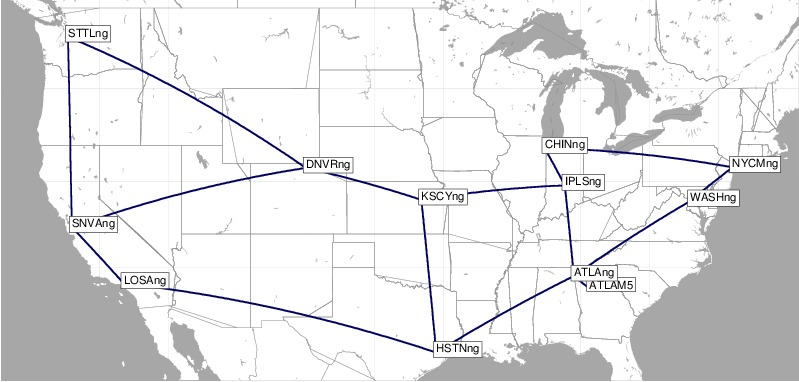
\includegraphics[width=0.8\textwidth]{pictures/abilene.jpg}
\caption[Topología Abilene]{Topología de Abilene.\\Fuente: SNDlib.}
\label{fig:topologia_abilene}
\end{figure}

\subsection{Emisiones de cada matriz de tráfico}

Previo a mostrar los resultados obtenidos de las pruebas realizadas, es importante conocer cuáles son las emisiones de la red con todos los enlaces encendidos para poder evaluar correctamente las mejoras alcanzadas. En la \autoref{fig:max_emisiones_abilene} se puede observar que las emisiones de la red son mayores a medida que aumenta el tráfico, pues el grado de utilización de los enlaces es un factor que influye bastante. Un detalle a tener en cuenta es que las emisiones mostradas en la gráfica no comienzan en cero, esto se ha hecho para observar claramente las diferencias entre cada matriz de tráfico.

\begin{figure}[H]
\centering
\captionsetup{justification=centering}
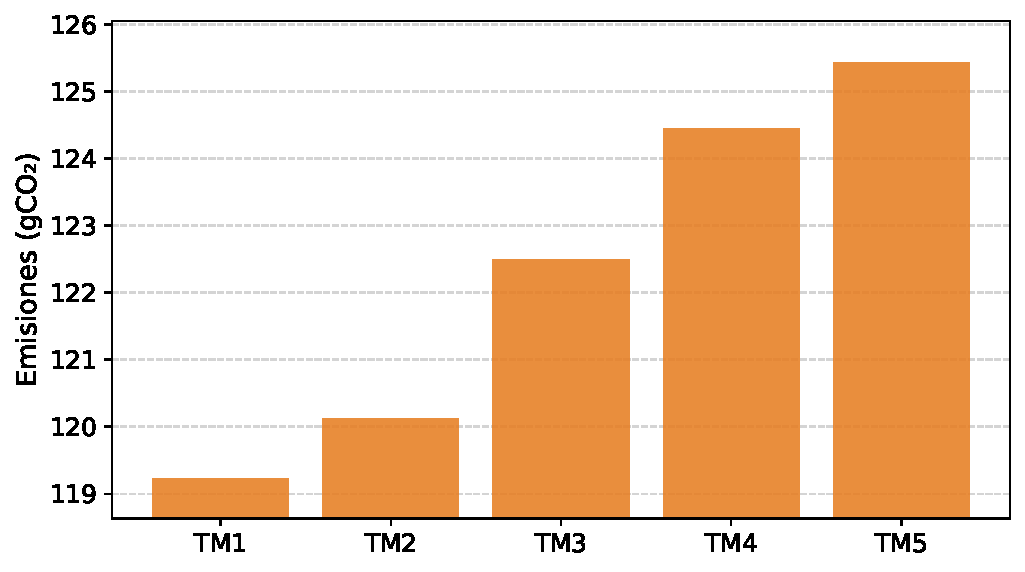
\includegraphics[width=0.6\textwidth]{pictures/max_carbon_Abilene.pdf}
\caption[Emisiones máximas Abilene]{Emisiones de Abilene con todos los enlaces encendidos.\\Fuente: Elaboración propia.}
\label{fig:max_emisiones_abilene}
\end{figure}

\subsection{Emisiones después del apagado de enlaces}

Las primeras pruebas que se realizaron con Abilene arrojaron unos resultados realmente prometedores. Haciendo uso de PSO normal con 200 partículas, 1200 iteraciones y 20 ejecuciones por cada matriz de tráfico, se han reducido las emisiones en hasta un 38.44\%. Además, como se muestra en la \autoref{fig:abilene_pso_20runs}, los intervalos de confianza son muy estrechos, lo que indica que con 20 ejecuciones el algoritmo presenta poca variabilidad y converge hacia soluciones de calidad.

\begin{figure}[H]
\centering
\captionsetup{justification=centering}
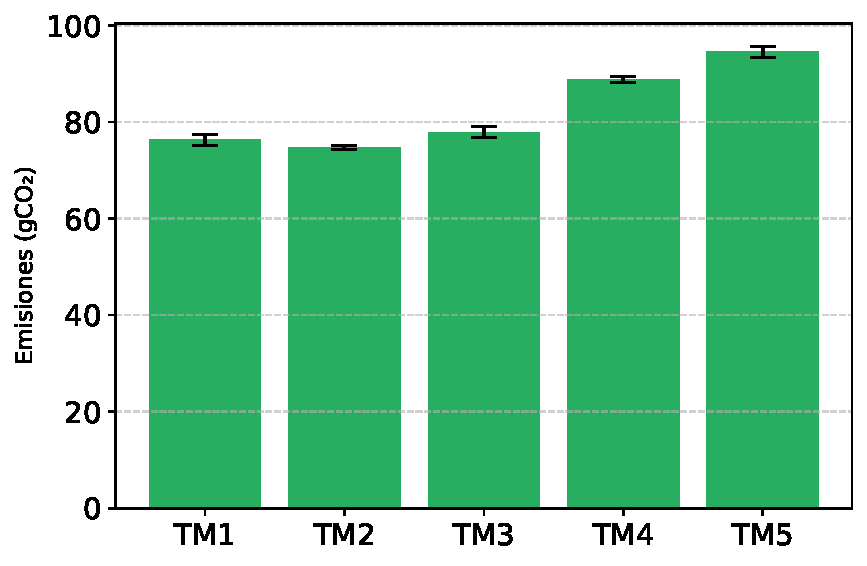
\includegraphics[width=0.6\textwidth]{pictures/abilene_pso_p200_i1200_c1-1.75_c2-2.25_w0.7_k100_20runs.pdf}
\caption[Resultados Abilene PSO 200p 1200i 20runs]{Emisiones de Abilene tras ejecutar PSO normal 20 veces por TM con 200 patículas y 1200 iteraciones. Intervalos de confianza al 95\%\\Fuente: Elaboración propia.}
\label{fig:abilene_pso_20runs}
\end{figure}

Al ejecutar el algoritmo 100 veces por cada matriz de tráfico con la misma configuración, los resultados que se muestran en la \autoref{fig:abilene_pso_100runs} son básicamente idénticos que los obtenidos en la prueba anterior. Lo único que cambia son los intervalos de confianza, que son aún más estrechos, lo que confirma el buen funcionamiento del algoritmo y su convergencia hacia soluciones de calidad.

\begin{figure}[H]
\centering
\captionsetup{justification=centering}
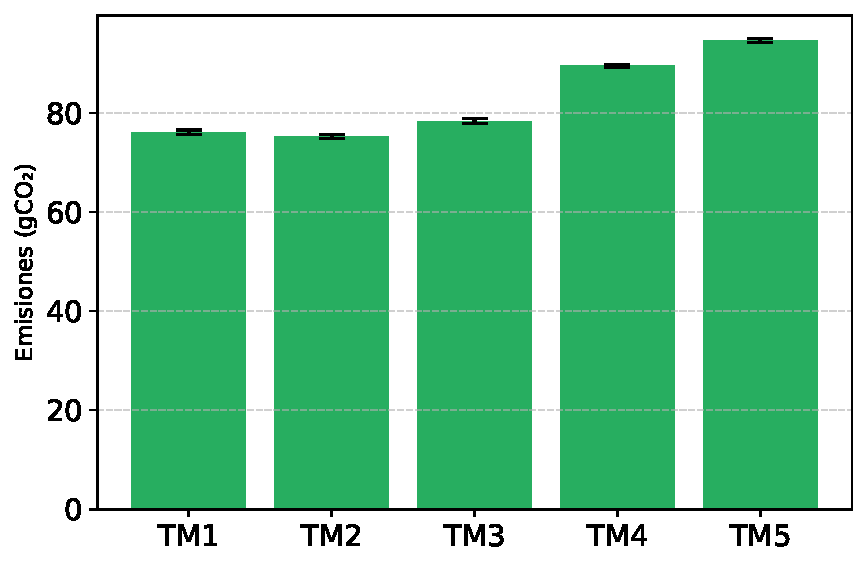
\includegraphics[width=0.6\textwidth]{pictures/abilene_pso_p200_i1200_c1-1.75_c2-2.25_w0.7_k100_100runs.pdf}
\caption[Resultados Abilene PSO 200p 1200i 100runs]{Emisiones de Abilene tras ejecutar PSO normal 100 veces por TM con 200 patículas y 1200 iteraciones. Intervalos de confianza al 95\%\\Fuente: Elaboración propia.}
\label{fig:abilene_pso_100runs}
\end{figure}

Tras estas primeras pruebas, se repitieron los experimentos manteniendo la configuración pero esta vez usando PSO VCH. Los resultados usando esta segunda estrategia son sorprendentes, pues se consigue una mejora de hasta un 20.80\% con respecto a PSO normal. En la \autoref{fig:abilene_vch_200p_1200i_20runs} se muestran estos incrementos de calidad en las soluciones, donde, además, se pueden observar unos intervalos de confianza muy estrechos, reforzando una vez más la estabilidad del algoritmo.

\begin{figure}[H]
\centering
\captionsetup{justification=centering}
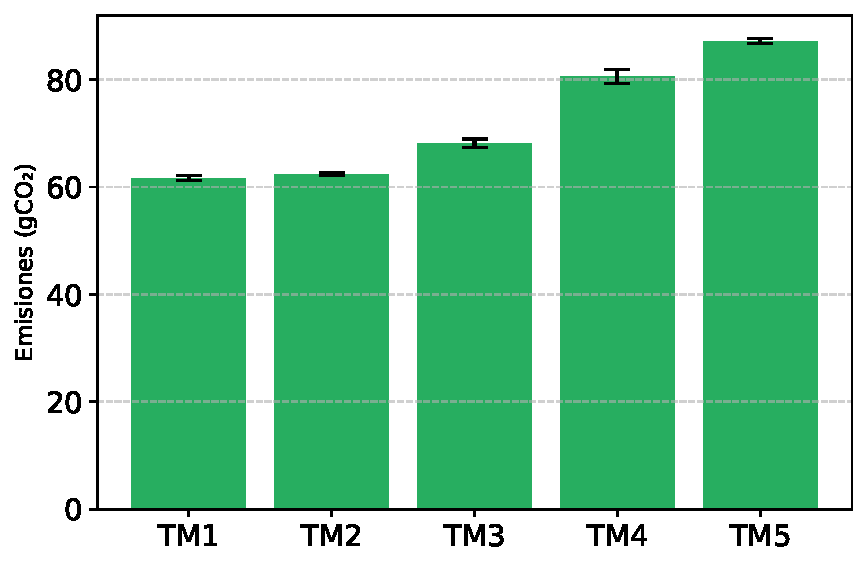
\includegraphics[width=0.6\textwidth]{pictures/abilene_vch_p200_i1200_c1-1.75_c2-2.25_w0.7_k100_20runs.pdf}
\caption[Resultados Abilene PSO VCH 200p 1200i 20runs]{Emisiones de Abilene tras ejecutar PSO VCH 20 veces por TM con 200 patículas y 1200 iteraciones. Intervalos de confianza al 95\%\\Fuente: Elaboración propia.}
\label{fig:abilene_vch_200p_1200i_20runs}
\end{figure}

Estas mejoras al usar PSO VCH con 200 partículas y 1200 iteraciones, inevitablemente plantean diferentes cuestiones: si se reducen las partículas a 100 ¿cuánto mejoran los tiempos de ejecución? ¿Se mantendría la calidad de los resultados? ¿Y si además se reducen las iteraciones a 600? Todas estas preguntas se responden durante las dos siguientes pruebas: primero, se redujeron las partículas a 100 manteniendo las 1200 iteraciones, y posteriormente, las iteraciones se fijaron en 600.

\begin{figure}[H]
    \centering
    \captionsetup{justification=centering}
    \begin{subfigure}{0.48\textwidth}
        \captionsetup{justification=centering}
        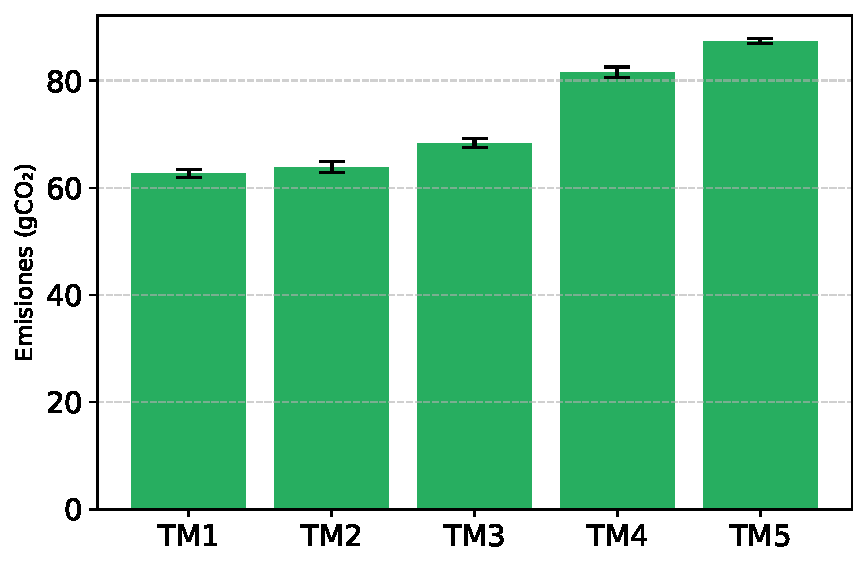
\includegraphics[width=\textwidth]{pictures/abilene_vch_p100_i1200_c1-1.75_c2-2.25_w0.7_k100_20runs.pdf}
        \caption[Resultados Abilene PSO VCH 100p 1200i 20runs]{Emisiones para 1200 iteraciones y 100 partículas.\\Fuente: Elaboración propia.}
        \label{fig:abilene_vch_100p_1200i}
    \end{subfigure}
    \hfill
    \begin{subfigure}{0.48\textwidth}
        \captionsetup{justification=centering}
        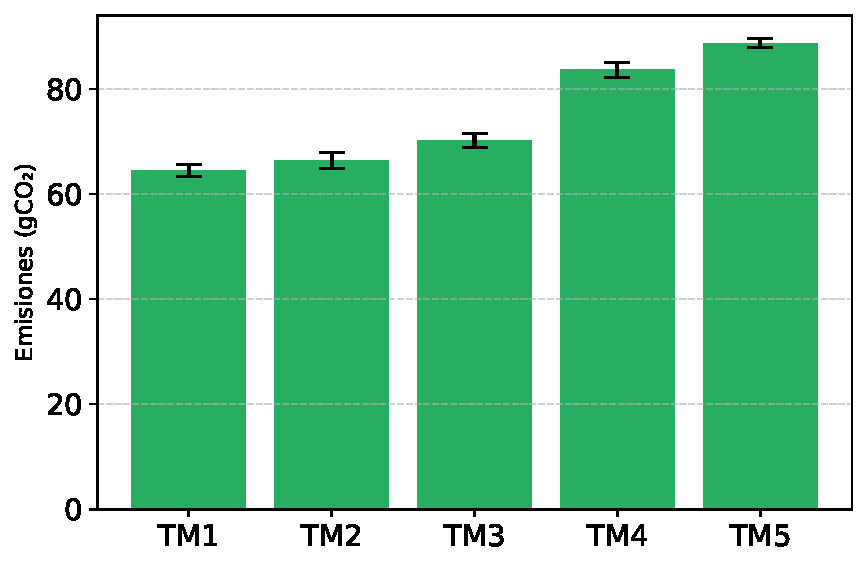
\includegraphics[width=\textwidth]{pictures/abilene_vch_p100_i600_c1-1.75_c2-2.25_w0.7_k100_20runs.pdf}
        \caption[Resultados Abilene PSO VCH 100p 600i 20runs]{Emisiones para 600 iteraciones y 100 partículas.\\Fuente: Elaboración propia.}
        \label{fig:abilene_vch_100p_600i}
    \end{subfigure}
    \caption[Resultados Abilene PSO VCH 100p]{Emisiones de Abilene tras ejecutar PSO VCH 20 veces por TM modificando partículas e iteraciones. Intervalos de confianza al 95\%}
    \label{fig:abilene_vch_100p}
\end{figure}

Los resultados de estas dos pruebas pueden verse en la \autoref{fig:abilene_vch_100p}. Aunque las emisiones son ligeramente más altas que con 200 partículas, siguen siendo soluciones de buena calidad. Además, los intervalos de confianza están bastante ajustados, lo cual indica que el comportamiento del algoritmo reduciendo a la mitad tanto el número de partículas como la cantidad de iteraciones, sigue presentando muy poca variabilidad y mantiene su tendencia a soluciones de calidad. La mejora más significativa reside en los tiempos de ejecución, pero esto se verá en detalle más adelante en la \autoref{sec:tiempos_abilene}.

Por último, en la figura X se presenta una gráfica final donde se muestran los resultados obtenidos con anterioridad, así como las emisiones de Abilene con todos los enlaces encendidos. De esta manera, de un solo vistazo se pueden comparar todos los resultados y observar las mejoras que se obtienen con cada configuración.

\subsection{Tiempos de ejecución} \label{sec:tiempos_abilene}

\begin{figure}[H]
\centering
\captionsetup{justification=centering}
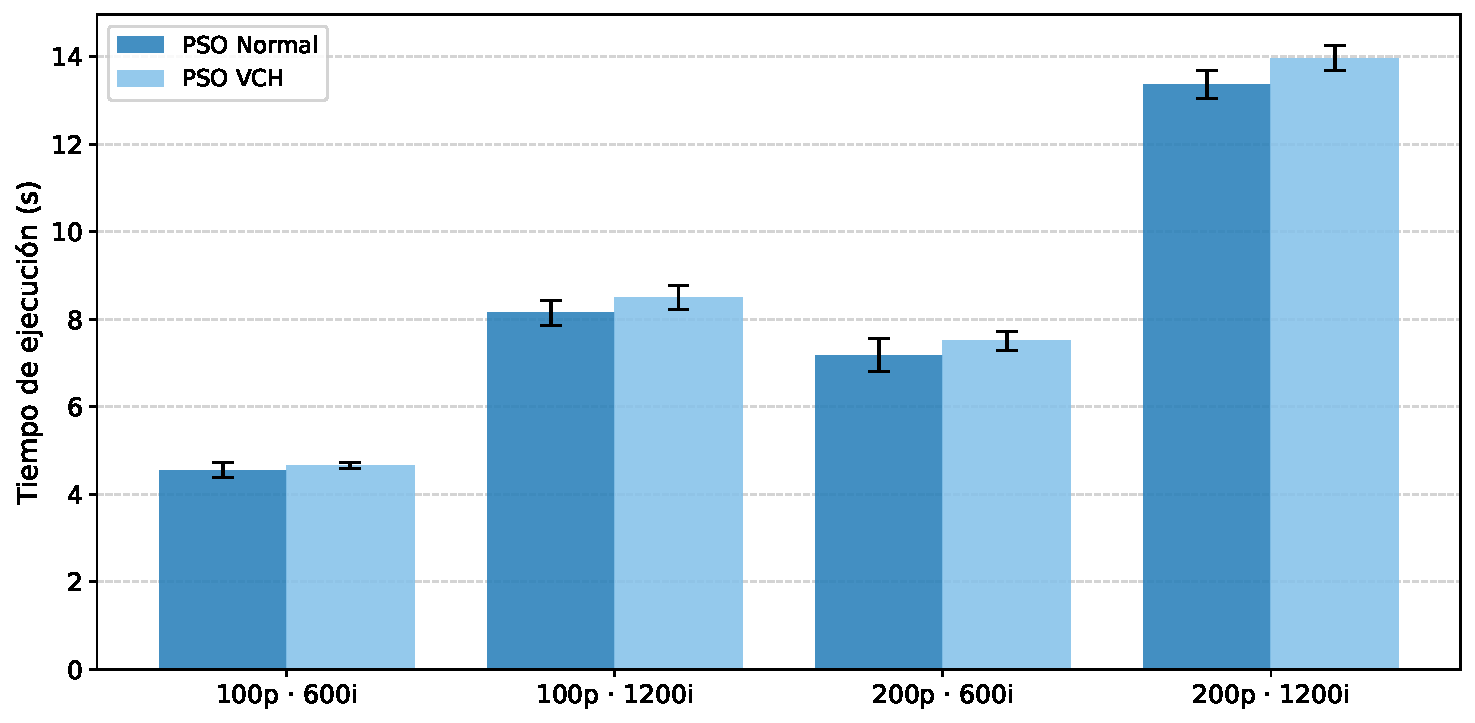
\includegraphics[width=0.7\textwidth]{pictures/tiempo_Abilene_partGroup.pdf}
\caption[Tiempos ejecución Abilene]{Tiempos de ejecución de Abilene. Intervalos de confianza al 95\%\\Fuente: Elaboración propia.}
\label{fig:abilene_tiempos}
\end{figure}

\subsection{Porcentaje de enlaces apagados}

\subsection{Ocupación de los enlaces tras el apagado}

\section{Resultados de Nobel y Geant}

\section{Análisis de Germany y limitaciones encontradas}